In this chapter, the theoretical model for \ac{ap} axis alignment is described. The chapter is divided into three sections. The first section reviews the model of \ac{ap} axis establishment described in \cite{gross2019guiding}, which utilizes a reaction-diffusion-advection system to describe the distribution of \ac{par} proteins and \ac{nmy2}. The second section reviews the model of the formation of pseudocleavage furrow via compressive alignment of actin filaments due to flows in the actomyosin cortex, as described in \cite{reymann2016cortical}. The third section describes the theoretical model of \ac{ap} axis alignment used in this thesis, by combining the two models discussed in the sections before. It also describes the details of the numerical simulations of the theoretical model, and how the parameters of the model were calibrated using experimental data. The theoretical model was developed in collaboration with M. Nestler and A. Voigt, with numerical simulations and calibration done by M. Nestler -- further details on the model are described in \cite{}.

\section{A model of \acs{ap} axis establishment in \acs{ce}}\label{sec:apAxisEstablishModelPG}
As discussed in \autoref{sec:ApAxisEstablishment}, the centrosomes associated with the male pronucleus guide the establishment of \ac{ap} axis. In \cite{gross2019guiding}, the authors propose a model to investigate the centrosome-guided \ac{ap} axis establishment. In particular, the following components are included in the model proposed in \cite{gross2019guiding}:
\begin{itemize}
    \item Mutual antagonism between \ac{apar} and \ac{ppar} \citep{hoege2013principles} is captured via a mass-conserved Turing-like system \citep{goehring2011advectionpolarization,lee2015self,halatek2018rethinking}
    \item Mechanochemical feedback between the \ac{par} polarity system and actomyosin cortex is captured via coupling this Turing-like system to an active isotropic fluid description of the cortex \citep{mayer2010anisotropies,bois2011pattern}
    \item Spatiotemporal cues provided by the centrosomes associated with the male pronucleus (for loading of \ac{ppar} and depletion of myosin on the cortex) are captured as two distinct guiding cues -- \ac{ppar} stabilization cue and actomyosin cue, with the latter having two components.
\end{itemize}
This section describes this model of \ac{ap} axis establishment introduced in \cite{gross2019guiding}. This model assumes that the male pronucleus is always present at the posterior end, and thus assumes rotational symmetry around the long axis of the embryo. This simplifies the model to a 1-dimensional model of length $L$ with periodic boundary conditions, along the boundary of the cross-section at the midplane of the embryo \citep{gross2019guiding}. The posterior end is considered to be at the center of the domain $x \in [-\frac{L}{2},\frac{L}{2}]$ -- that is, at $x = 0$ (see \autoref{fig:apAxisEstablishModelPG}). Note that the curvature of the embryo boundary is neglected in this model.

\begin{figure}
\centering
\begin{subfigure}{\textwidth}
    \centering
    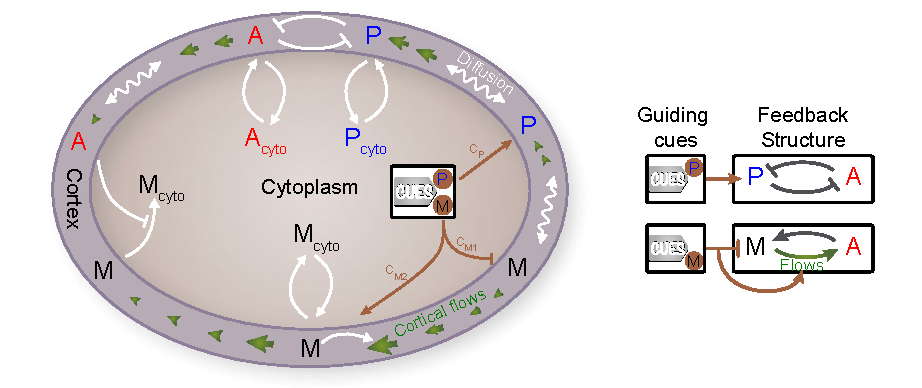
\includegraphics[width=\textwidth]{ActiveMatterModel/FigureModelPG/modelPG.pdf}
    \caption{Schematic depicting the Turing-like system for \ac{apar} $A$, \ac{ppar} $P$ and myosin $M$. These proteins are either located in the cytoplasm (denoted using the $cyto$ subscript) or at the cortex, where they are subjected to lateral diffusion and advective transport by cortical flows. The following reactions are considered: spontaneous association with and dissociation from the cortex, mutual antagonism between \ac{apar} and \ac{ppar} when associated to the cortex, and \ac{apar} regulated dissociation of myosin from the cortex. Two guiding cues are provided by the centrosomes and steer the \ac{ap} axis establishment process: \ac{ppar} domain stabilisation cue (denoted by $c_P$) and actomyosin cue with two components -- one depleting myosin at the cortex (denoted by $c_{M1}$) and the other regulating contractility (denoted by $c_{M2}$. See \autoref{sec:apAxisEstablishModelPG} for details.}
    \label{subfig:apAxisEstablishModelPG-schematic}
\end{subfigure}
\hfill
\begin{subfigure}{\textwidth}
    \centering
    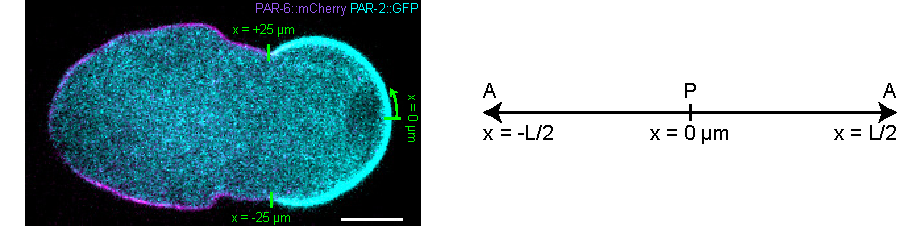
\includegraphics[width=\textwidth]{ActiveMatterModel/FigureModelPG/par2Par6SymmetricArclength.pdf}
    \caption{Left: Mid-plane section of the \acs{ce} embryo, labelled with PAR-2::\ac{gfp} (posterior domain, in cyan) and PAR-6::mCherry (anterior domain, in magenta). The model discussed in \autoref{sec:apAxisEstablishModelPG}, using the rotational symmetry around the long axis, is reduced to a 1-dimensional model along the boundary of this mid-plane section, endowned with the arclength variable $x$. $x$ is annotated in green -- $x = 0$ denotes the posterior pole. Scale bar: \SI{10}{\micro\meter}. Note that the positive and negative \enquote{arm} of the boundary is flipped compared to that in \cite{gross2019guiding} following the convention followed in this thesis. Right: Boundary of the cross-section at the midplane of the embryo reduced to a 1-dimensional line with periodic boundary conditions. $x = 0$ is at the posterior pole (denoted by P), and $x = \pm \flatfrac{L}{2}$ at the anterior (denoted by A).}
    \label{subfig:apAxisEstablishModelPG-arclengthMidplaneBoundary}
\end{subfigure}
\caption[Schematic representing the \acs{ap} axis establishment model in \cite{gross2019guiding}]{Schematic representing the 1-dimensional model of \acs{ap} axis establishment described in \cite{gross2019guiding}, and visualization of the arclength axis used in the model. Figure adapted froim \cite{gross2019guiding}, see \autoref{sec:apAxisEstablishModelPG} for details}
\label{fig:apAxisEstablishModelPG}
\end{figure}

\subsection{Turing-like system for \acs{par} polarity system}\label{subsec:parPolarityReactionDiffusionAdvectionModelPG}
Three proteins are considered in the model discussed in this section: \ac{apar}, \ac{ppar} and myosin. Each protein has a membrane-bound fraction and a cytoplasmic fraction, with exchange between the two fractions throughout the cortex. It is assumed that the sum total of its membrane-bound fraction $c$ and cytoplasmic fraction $c_{cyto}$ is a constant $c_{tot}$ throughout the \ac{ap} axis establishment. Here $c$ can either be $A,P$ or $M$ -- representing \ac{apar}, \ac{ppar} or myosin respectively. This constraint of limited protein pool can be written as:
\begin{equation}
    c_{tot} V = \int_{\textrm{cortex}} c \dd{S} + \int_{\textrm{cytoplasm}} c_{cyto} \dd{V}
\end{equation}
where $V$ is the volume of the embryo and $c, c_{cyto}$ are volumetric concentrations while $c$ is surface concentration of the protein considered. It is further assumed that the cytoplasmic concentrations are fairly homogeneous (therefore, $\int_{\textrm{cytoplasm}} c_{cyto} \dd{V} \approx c_{cyto} V$)  -- due to the large diffusion coefficients in the cytoplasm \citep{goehring2011proteins}. Altogether, this leads to the following expression for the concentration of the cytoplasmic fraction $c_{cyto}$:
\begin{equation}
    c_{cyto} = c_{tot} - \frac{1}{V}\int_{\textrm{cortex}} c \dd{S}
\end{equation}
In the model discussed in this section, rotational symmetry has been used to reduce the cortex to a 1-dimensional surface along the embryo boundary at the mid-plane cross-section. In this scenario, the above reduces to:
\begin{equation}\label{eq:concCytoModelPG}
    c_{cyto} = c_{tot} - \frac{\psi}{L}\int^{\frac{L}{2}}_{-\frac{L}{2}} c(x,t) \dd{S}
\end{equation}
where $\psi$ is the surface-to-volume ratio for the ellipsoidal geometry of the embryo.

The spatiotemporal dynamics of the surface concentrations $c$ are considered next. The continuity equation for $c$ can be written as (from \autoref{eq:introSpeciesBalance}):
\begin{equation}
    \inlinePartial{t}{c}(x,t) + \inlinePartial{x}{\speciesSuper{J}{c}} = \speciesSuper{r}{c}
\end{equation}
where $\speciesSuper{J}{c}$ is the flux of proteins $c$ and $\speciesSuper{r}{c}$ the rate of generation of $c$ from all the reactions that affect $c$. As before, $\speciesSuper{J}{c} = cv + \speciesSuper{j}{c}$ can be split into a advective flux (due to advection with cortical flow velocity $\vec{v}(x,t)$) and relative flux $\speciesSuper{j}{c}$. In the model discussed here, the relative flux $\speciesSuper{j}{c}$ arises due to passive diffusion -- thus, $\speciesSuper{j}{c} = -D_c\inlinePartial{x}{c}$ from Fick's law of diffusion, for diffusion constant $D_c$. Altogether, the dynamics of $c(x,t)$ is given by:
\begin{equation}\label{eq:concDynamicsModelPG}
    \inlinePartial{t}{c}(x,t) = -\inlinePartial{x}{(cv)} + D_c\inlinePartial[2]{x}{c} + \speciesSuper{r}{c} 
\end{equation}
for $c$ being either $A,P$ or $M$. \autoref{eq:concDynamicsModelPG} includes three physical processes: advective transport by cortical flows $-\inlinePartial{x}{(cv)}$, passive diffusion on the cortex $D_c\inlinePartial[2]{x}{c}$ and chemical reactions amongst the surface-bound molecules and their cytoplasmic counterparts. The reaction terms $\speciesSuper{r}{c}$ are considered next.

For myosin, two reactions are considered: exchange of cortical myosin with the cytoplasm, and regulation of the dissociation rate (from the cortex) by \ac{apar} \citep{gross2019guiding}. The reaction rate $\speciesSuper{r}{M}$ can then be written as:
\begin{equation}\label{eq:myosinChemicalRateModelPG}
    \speciesSuper{r}{M} = k_{on,M}M_{cyto} - \left[k_{off,M} - k_{AM}A\right]M
\end{equation}
where $k_{on,M}$ and $k_{off,M}$ are myosin association (to the cortex) and dissociation (from the cortex) rates -- governing the exchange between the cortical and cytoplasmic myosin. $k_{AM}$ represents the regulation of the dissociation rate of myosin by \ac{apar}.

For \ac{apar} and \ac{ppar}, two reactions are considered: exchange with cytoplasmic bulk fraction, and mutual antagonism on the cortex between \ac{apar} and \ac{ppar} \citep{hoege2013principles}. For \ac{apar}, this antagonism occurs in the form of regulation of the cortical association rate of \ac{apar} by the \ac{ppar} protein complex \citep{robin2014single,sailer2015dynamic}. For \ac{ppar}, this antagonism instead occurs in the form of regulation of the cortical dissociation rate of \ac{ppar} by the \ac{apar} protein complex \citep{goehring2011advectionpolarization}. Thus, including both exchange with the cytoplasm and mutual antagonism in the \ac{par} polarity system, the reaction rates $\speciesSuper{r}{A}$ and $\speciesSuper{r}{P}$ can be written as:
\begin{subequations} \label{eq:parChemicalRateModelPG}
    \begin{align}
        \speciesSuper{r}{A} &= \frac{k_{on,A}}{1 + k_{AP}P^{s_P}}A_{cyto} - k_{off,A}A\\
        \speciesSuper{r}{P} &= k_{on,P}P_{cyto} - \left[k_{off,P} + k_{PA}A^{s_A}\right]P
    \end{align}
\end{subequations}
where $k_{on,A}$ and $k_{off,A}$ are association and dissociation rates for \ac{apar}, and similarly $k_{on,P}$ and $k_{off,P}$ are association and dissociation rates for \ac{ppar}. These govern the exchange between the cortical and cytoplasmic fractions of the \ac{par} proteins. $k_{AP}$ and $k_{PA}$ represents the mutual antagonism between \ac{apar} and \ac{ppar} proteins, and $s_A$ and $s_P$ are stoichiometric coefficients.

\subsection{Active isotropic description of actomyosin cortex}\label{subsec:actomyosinCortexModelPG}
In the model described in this section, the actomyosin cortex is considered as an active isotropic fluid, with an additional frictional drag force on the cortex due to the surrounding cell membrane, eggshell and cytoplasm \citep{mayer2010anisotropies}. In other words, the momentum balance in this model is written as:
\begin{equation}\label{eq:momentumBalanceModelPG}
    \inlinePartial{\beta}{\sigma_{\alpha\beta}} - \gamma v_\alpha = 0
\end{equation}
where $\gamma$ is the frictional drag coefficient. As the flows in the actomyosin cortex may be considered to in the low-reynolds number regime, the inertial term $\rho(\inlinePartial{t}{v_\alpha} + v_\beta\inlinePartial{\beta}{v_\alpha})$ from \autoref{eq:introMomentumBalanceVelocityForm} can be neglected. 

Furthermore, the stress is separated into a passive viscous stress and an active actomyosin-generated stress. Namely, \autoref{eq:introActiveSimpleFluidStress} may be re-written as (for the 2-dimensional cortex):
\begin{equation}\label{eq:totalStressModelPG}
    \sigma_{\alpha\beta} = \left[2\eta \left(\frac{\inlinePartial{\beta}{v_\alpha} + \inlinePartial{\alpha}{v_\beta}}{2} - \frac{1}{2}\inlinePartial{\gamma}{v_\gamma}\delta_{\alpha\beta}\right) + \left(\eta_v\inlinePartial{\gamma}{v_\gamma} - p\right)\delta_{\alpha\beta}\right] + \zeta\Delta\mu \delta_{\alpha\beta} = \speciesSuper{\sigma}{passive}_{\alpha\beta} + \speciesSuper{\sigma}{active}_{\alpha\beta}
\end{equation}
where $\speciesSuper{\sigma}{passive}_{\alpha\beta} = 2\eta \left(\frac{\inlinePartial{\beta}{v_\alpha} + \inlinePartial{\alpha}{v_\beta}}{2} - \frac{1}{2}\inlinePartial{\gamma}{v_\gamma}\delta_{\alpha\beta}\right) + \left(\eta_v\inlinePartial{\gamma}{v_\gamma} - p\right)\delta_{\alpha\beta}$ contains all the viscous terms in the stress and $\speciesSuper{\sigma}{active}_{\alpha\beta} = \zeta\Delta\mu \delta_{\alpha\beta}$ is the active stress generated by myosin motors. Here, $\eta$ and $\eta_v$ are shear and bulk viscosity coefficients, $p$ is the pressure, $\Delta\mu$ the difference in chemical potential for \ac{atp} hydrolysis and $\zeta$ is a phenomenological coefficient that denotes the stress generated by myosin motors. Note that rotational symmetry has not been utilized till now, in the description of the cortex.

Following \cite{julicher2018hydrodynamic}, the passive viscous stress may be written as:
\begin{equation}
    \speciesSuper{\sigma}{passive}_{\alpha\beta} = 2\eta \left(\frac{\inlinePartial{\beta}{v_\alpha} + \inlinePartial{\alpha}{v_\beta}}{2} - \frac{1}{2}\inlinePartial{\gamma}{v_\gamma}\delta_{\alpha\beta}\right) + \left(\eta_v\inlinePartial{\gamma}{v_\gamma} - p\right)\delta_{\alpha\beta}
\end{equation}
where $\bar{\eta}$ is effective 2-D bulk viscosity of the cortex. In the the model described here, this effective bulk viscosity is neglected -- thus, only the shear stress related term is retained. Rotational symmetry around the long axis implies that gradients survive only along the x-axis, thus reducing the passive viscous stress to:
\begin{equation}\label{eq:passiveStressModelPG}
    \speciesSuper{\sigma}{passive} = \eta \inlinePartial{x}{v}
\end{equation}
The active stress $\speciesSuper{\sigma}{active}$ is assumed to be of the following form:
\begin{equation}\label{eq:activeStressModelPG}
    \speciesSuper{\sigma}{active} = C_*\frac{M}{M + M_*}
\end{equation}
where $C_*$ indicates the strength of cortical contractility, $M$ is the local concentration of myosin and $M_*$ is a Hill coefficient. Note that $M_*$ controls the sensitivity of active stress to myosin concentration -- if $M >> M_*$, $\speciesSuper{\sigma}{active} \approx C_*$, while if $M << M_*$, $\speciesSuper{\sigma}{active} \approx \frac{C_*}{M_*}$. In other words, a myosin rich patch of cortex generates an active stress closer to $C_*$, while a myosin poor patch generates a much smaller active stress closer to $\frac{C_*}{M_*}$.

\subsection{Guiding cues for \acs{ap} axis establishment}\label{subsec:guidingCuesModelPG}
Before the dynamical equations for the concentrations $c(x,t) = A,P,M$ and cortical velocity $v(x,t)$ are written, the guiding cues provided by the centrosome need to be considered. Since in the model described in this section, it is assumed that the male pronucleus is at the posterior end, these cues are provided at the posterior pole -- that is, at $x = 0$. Two guiding cues are provided by the centrosomes -- a cue to the \ac{ppar} domain, and a cue to the actomyosin cortex. Additionally, the cue to the actomyosin cortex contains two components. Altogether, these cues are:
\begin{itemize}
    \item \ac{ppar} domain stabilisation cue, due to the microtubule-mediated local inhibition of removal of \ac{ppar} from the cortex by \ac{apar} \citep{motegi2011microtubules}. This cue is incorporated in the model by modifying the reaction rate for \ac{ppar} $\speciesSuper{r}{P}$ as:
    \begin{equation}\label{eq:pparChemicalRateWithCueModelPG}
        \speciesSuper{r}{P} = k_{on,P}P_{cyto} - \left[k_{off,P} + k_{PA}A^{s_A}(1 - \kappa_PF_P(x)f_P(t))\right]P
    \end{equation}
    where $\kappa_P$ is the (dimensionless) strength of the \ac{ppar} domain stabilisation cue. $F_P(x)$ localizes the cue near the posterior pole -- and selected to be a gaussian $F_p(x) = \exp(-\frac{x^2}{d_P^2})$ with characteristic length $d_P$. $f_P(t)$ captures the temporal characteristics of the cue, and is set to $f_P(t) = \frac{1}{2}\left[\tanh(\frac{t}{\tau_{P,on}}) + 1\right]$. $f_P(t)$ describes a smooth transition from zero at $t = 0$ to one on the time-scale $\tau_{on,P}$. The \ac{ppar} domain stabilisation cue thus starts at $t = 0$ and remains on.
    \item Myosin depletion component of the actomyosin cue, acting via an unknown mechanism \citep{motegi2006sequential}. This cue is incorporated in the model by modifying the reaction rate for myosin $\speciesSuper{r}{M}$ as:
    \begin{equation}\label{eq:myosinChemicalRateWithCueModelPG}
        \speciesSuper{r}{M} = k_{on,M}M_{cyto} - \left[k_{off,M}(1 + \kappa_MF_M(x)f_M(t)) - k_{AM}A\right]M
    \end{equation}
    where $\kappa_M$ is the (dimensionless) strength of the actomyosin cue. $F_M(x)$ localizes the cue near the posterior pole -- and selected to be a gaussian $F_M(x) = \exp(-\frac{x^2}{d_M^2})$ with characteristic length $d_M$. $f_M(t)$ captures the temporal characteristics of the cue, and is set to $f_M(t) = \frac{1}{2}\left[\tanh(\frac{t}{\tau_{M,on}}) - \tanh(\frac{t - T_M}{\tau_{M,off}})\right]$. $f_M(t)$ describes a smooth transition from zero at $t = 0$ to one on the time-scale $\tau_{on,M}$, and subsequently from one to zero after $t = T_M$ on a time-scale $\tau_{off,M}$. The myosin depletion component of the actomyosin cue thus starts at $t = 0$ and remains active until $t = T_M$, after which it shuts off.
    \item Contractility component of the actomyosin cue, due to the up-regulation of myosin contractility briefly after centrosomes trigger polarity establishment \citep{tse2012nop1}. This cue is incorporated in the model by modifying the active stress $\speciesSuper{\sigma}{active}$ as:
    \begin{equation}\label{eq:activeStressWithCueModelPG}
        \speciesSuper{\sigma}{active} = C_*f_C(t)\frac{M}{M + M_*}
    \end{equation}
    where $f_C(t)$ captures the temporal characteristics of the cue, and is set to $f_C(t) = \frac{1}{2}\left[1 - \tanh(\frac{t-T_M}{\tau_{M,off}})\right]$. $f_C(t)$ describes a smooth transition from one to zero after $t = T_M$ on a time-scale $\tau_{off,M}$. The contractility component of the actomyosin cue thus turns off after $t = T_M$.
\end{itemize}

\subsection{Full model of \acs{ap} axis establishment in \citep{gross2019guiding}}\label{subsec:fullModelPG}
Combining all these together, the full set of dynamic equations for the concentrations\\ $A(x,t),P(x,t),M(x,t)$ (for \ac{apar}, \ac{ppar} and myosin respectively) are given by:
\begin{subequations}\label{eq:allConcDynamicsModelPG}
    \begin{align}
        \inlinePartial{t}{A} &= -\inlinePartial{x}{(vA)} + D_A\inlinePartial[2]{x}{A} + \frac{k_{on,A}}{1 + k_{AP}P^{s_P}}A_{cyto} - k_{off,A}A\\
        \inlinePartial{t}{P} &= -\inlinePartial{x}{(vP)} + D_P\inlinePartial[2]{x}{P} + k_{on,P}P_{cyto} - \left[k_{off,P} + k_{PA}A^{s_A}(1 - \kappa_PF_P(x)f_P(t))\right]P\\
        \inlinePartial{t}{M} &= -\inlinePartial{x}{(vM)} + D_M\inlinePartial[2]{x}{M} + k_{on,M}M_{cyto} - \left[k_{off,M}(1 + \kappa_MF_M(x)f_M(t)) - k_{AM}A\right]M
    \end{align}
\end{subequations}
where $v(x,t)$ is the cortical flow velocity, and the rest of the terms are defined as in \autoref{subsec:parPolarityReactionDiffusionAdvectionModelPG} and \autoref{subsec:guidingCuesModelPG}. The cytoplasmic concentrations $A_{cyto}, P_{cyto}, M_{cyto}$ are found using \autoref{eq:concCytoModelPG}.

The dynamical equation for cortical flow velocity $v(x,t)$ is written using the momentum balance (\autoref{eq:momentumBalanceModelPG}) and the definitions of active (\autoref{eq:activeStressWithCueModelPG}) and passive stresses (\autoref{eq:passiveStressModelPG}) as:
\begin{equation}\label{eq:velocityDynamicsModelPG}
    \eta \inlinePartial[2]{x}{v} - \gamma v = -C_*f_C(t)\inlinePartial{x}{\left(\frac{M}{M + M_*}\right)}
\end{equation}
where $\eta$ is the viscosity of the cortex and $\gamma$ the frictional drag coefficient. $C_*$ and $M_*$ are defined in \autoref{subsec:actomyosinCortexModelPG}, and $f_C(t)$ in \autoref{subsec:guidingCuesModelPG}.

\section{A model of pseudocleavage furrow formation in \acs{ce}}\label{sec:furrowFormationModelAC}
In \cite{reymann2016cortical}, the authors investigate the role of cortical flows in the formation of contractile rings in the \ac{ce} embryo, such as the pseudocleavage furrow or the cytokinetic ring. The pseudocleavage furrow, as mentioned in \autoref{sec:ApAxisEstablishment}, is a contractile ring-like structure that appears late in the establishment phase which appears as a furrow in the middle of the embryo \citep{nigon1960architecture,reymann2016cortical}. The cytokinetic ring is a contractile ring that forms much later during the first cell division in the embryo, and divides the one-cell P0 embryo into a larger AB cell and a smaller P1 cell (see \autoref{sec:CelegansModel}). The discussion here focuses on the pseudocleavage furrow only.

In \cite{reymann2016cortical}, the authors show that the contractile ring that is the pseudocleavage furrow forms as a result of cortical flow-driven compressive alignment of actin filaments in the actomyosin cortex. For this purpose, the authors in \cite{reymann2016cortical} propose a model of the actomyosin cortex as an active nematic fluid, which is discussed in this section. The nematic tensor $Q_{\alpha\beta}$ quantifies the average orientation of actin filaments in the cortex at the micrometer scale -- see the discussion on coarse-grained variables in \autoref{sec:introHydrodynamicTheoryActiveFluids}. The model considers the case where the male pronucleus is at the posterior pole of the embryo -- that is, when the \ac{ap} axis is aligned with the long axis of the embryo. Thus, the model assumes rotational symmetry around the long axis of the embryo, as was the case in the previous section. Additionally, the curvature of the embryo is neglected, allowing a description of the cortex in an effective Cartesian coordinate system (see \autoref{fig:pcFurrowXYAxisModelAC}).

\begin{figure}[h]
    \centering
    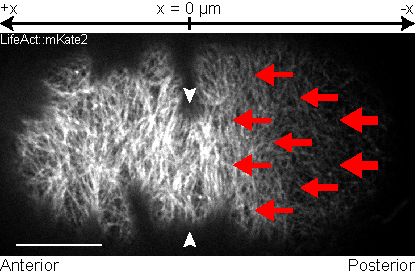
\includegraphics[width=0.7\textwidth]{ActiveMatterModel/FigureModelAC/pcFurrowXYAxis.pdf}
    \caption[Pseudocleavage furrow formation by compressive alignment of actin filaments]{Cortical section of the \acs{ce} embryo, labelled with LifeAct::mKate2 (white), to depict the organisation of actin filaments at onset of pseudocleavage furrow (white arrows). Red arrows depict anterior-directed cortical flows observed during pseudocleavage furrow onset. The $x$ axis used in \autoref{sec:furrowFormationModelAC} are also depicted, with $x = \SI{0}{\micro\meter}$ at the pseudocleavage furrow, and the posterior (anterior) on the negative (positive) $x$ end. $y$ axis is along the vertical edge of the image. Scale bar: \SI{10}{\micro\meter}. Adapted from \cite{reymann2016cortical}}
    \label{fig:pcFurrowXYAxisModelAC}
\end{figure}

\subsection{Dynamics of Actin alignment}\label{subsec:actinAlignmentModelAC}
Following the discussion in \autoref{sec:introHydrodynamicTheoryActiveFluids}, the constitutive equation that governs the rate of change in the nematic tensor for an active nematic fluid may be written from \autoref{eq:constitutiveEqActiveNematic} as:
\begin{equation}\label{eq:nematicDynamicsGeneralModelAC}
    \frac{DQ_{\alpha\beta}}{Dt} = -\nu \Tilde{v}_{\alpha\beta} + \frac{1}{\bar{\gamma}}H_{\alpha\beta} + \lambda Q_{\alpha\beta}\Delta\mu
\end{equation}
where $\frac{DQ_{\alpha\beta}}{Dt} = \inlinePartial{t}{Q_{\alpha\beta}} + v_\gamma\inlinePartial{\gamma}{Q_{\alpha\beta}} + \omega_{\alpha\gamma}Q_{\gamma\beta} + \omega_{\beta\gamma}Q_{\alpha\gamma}$ is the corotational and comoving derivative of $Q_{\alpha\beta}$ (see \autoref{eq:introCorotateDeriveQ}), $\Tilde{v}_{\alpha\beta} = \frac{\inlinePartial{\alpha}{v_\beta} + \inlinePartial{\beta}{v_\alpha}}{2} - \frac{1}{2}\inlinePartial{\gamma}{v_\gamma}\delta_{\alpha\beta}$ is the traceless symmetric part of the velocity gradient (written for a 2-dimensional cortex, see \autoref{eq:introActiveNematicStrainRate}), $\omega_{\alpha\beta} = \frac{\inlinePartial{\alpha}{v_\beta} - \inlinePartial{\beta}{v_\alpha}}{2}$ is the antisymmetric part of the velocity gradient (see \autoref{eq:introVorticityNematic}), $H_{\alpha\beta} = -\fdv{F_0}{Q_{\alpha\beta}}$ is the molecular field conjugate to the nematic tensor $Q_{\alpha\beta}$ for the instrinsic free energy $F_0$ (see \autoref{eq:introMolecularFieldDefine}) and $\Delta\mu$ is the chemical potential difference for \ac{atp} hydrolysis. Note that the corotational and comoving derivative $\frac{DQ_{\alpha\beta}}{Dt}$ includes the effect of advection on $Q_{\alpha}{\beta}$.

The phenomenological coefficient $\nu$ captures the change in nematic tensor $Q_{\alpha\beta}$ due to the velocity gradient $\Tilde{v}_{\alpha\beta}$ -- thus capturing the compressive alignment of actin filaments driven by flows in the actomyosin cortex. The phenomenological coefficient $\lambda$ couples the activity of myosin motors (which catalyse the hydrolysis of \ac{atp}) to the change in nematic tensor $Q_{\alpha\beta}$ -- thus capturing the active alignment of actin filaments by myosin motors. The phenomenological coefficient $\bar{\gamma}$ captures the relaxation of the actin alignment to the equilibrium state. For the free energy $F_0$, the following form is assumed:
\begin{equation}\label{eq:nematicFreeEnergyModelAC}
    F_0 = K\int\left[\frac{1}{2}Q_{\alpha\beta}Q_{\alpha\beta} + \frac{l^2}{2}\inlinePartial{\gamma}{Q_{\alpha\beta}}\inlinePartial{\gamma}{Q_{\alpha\beta}}\right]\dd{S}
\end{equation}
where the integral is taken over the whole cortex, $K$ characterises the tendency of actin filaments to relax to isotropic orientation ($K > 0$), and $l$ is the characteristic length scale below which filaments are coherently aligned. This form of $F_0$ yields $H_{\alpha\beta}$ as:
\begin{equation}\label{eq:molecularFieldModelAC}
    H_{\alpha\beta} = -\fdv{F_0}{Q_{\alpha\beta}} = K[l^2\inlinePartial{\gamma}{\inlinePartial{\gamma}{Q_{\alpha\beta}}} - Q_{\alpha\beta}]
\end{equation}

Finally, it is noted in \cite{reymann2016cortical} that the active alignment of actin filaments by myosin motors plays an insignificant role in the formation of the pseudocleavage furrow. Thus, $\lambda$ is set to zero. This yields the following equation for the dynamics of $Q_{\alpha\beta}$:
\begin{equation}\label{eq:nematicDynamicsPseudocleavageFurrowModelAC}
    \frac{DQ_{\alpha\beta}}{Dt} = -\nu \Tilde{v}_{\alpha\beta} + \frac{1}{\bar{\gamma}}H_{\alpha\beta} = -\nu \Tilde{v}_{\alpha\beta} + \frac{Kl^2}{\bar{\gamma}}\inlinePartial{\gamma}{\inlinePartial{\gamma}{Q_{\alpha\beta}}} - \frac{K}{\bar{\gamma}}Q_{\alpha\beta}
\end{equation}
As the model assumes the \ac{ap} axis is aligned with the long axis, the rotational symmetry around the long axis can be utilized to neglect derivatives in directions perpendicular to the long axis. Additionally, the component of the cortical flow velocity perpendicular to the long axis is also ignored. This simplifies \autoref{eq:nematicDynamicsPseudocleavageFurrowModelAC} into:
\begin{subequations}\label{eq:nematicDynamicsPseudocleavageFurrowAxiSymmetricModelAC}
    \begin{align}
        \inlinePartial{t}{Q_{xx}} + v_x\inlinePartial{x}{Q_{xx}} &=  -\frac{\nu}{2}\inlinePartial{x}{v_x} + \frac{Kl^2}{\bar{\gamma}}\inlinePartial[2]{x}{Q_{xx}} - \frac{K}{\bar{\gamma}}Q_{xx}\\
        \inlinePartial{t}{Q_{xy}} + v_x\inlinePartial{x}{Q_{xy}} &=  \frac{Kl^2}{\bar{\gamma}}\inlinePartial[2]{x}{Q_{xy}} - \frac{K}{\bar{\gamma}}Q_{xy}
    \end{align}
\end{subequations}
where $x$ denotes the direction along the long axis and $y$ perpendicular to it, on the cortex (see \autoref{fig:pcFurrowXYAxisModelAC}). Note that the curvature of the embryo is not considered in these equations. The nematic tensor is given by:
\begin{equation}
    Q_{\alpha\beta} = \begin{bmatrix} Q_{xx} & Q_{xy}\\ Q_{xy} & -Q_{xx} \end{bmatrix}
\end{equation}
Thus, given the cortical flow velocity $v_x$, \autoref{eq:nematicDynamicsPseudocleavageFurrowAxiSymmetricModelAC} governs the dynamics of the nematic tensor $Q_{\alpha\beta}$ and consequently the alignment of actin filaments in the cortex. At steady state, as assumed in \citep{reymann2016cortical}, $\inlinePartial{t}{Q_{xx}}$ and $\inlinePartial{t}{Q_{xy}}$ are set to zero.

\subsection{Active stress generated by alignment of actin filaments}\label{subsec:activeNematicStressModelAC}
In \cite{reymann2016cortical}, the following form for the stress tensor is proposed:
\begin{equation}\label{eq:totalStressModelAC}
    \sigma_{\alpha\beta} = \eta \Tilde{v}_{\alpha\beta} + \eta_v \inlinePartial{\gamma}{v_\gamma}\delta_{\alpha\beta} + \zeta \delta_{\alpha\beta} + \speciesSuper{\sigma}{nematic}_{\alpha\beta}
\end{equation}
where $\eta$ and $\eta_v$ are shear and bulk viscosity of the cortex respectively. $\zeta$ represents the isotropic part of the active contractile stresses generated by myosin motors in the actomyosin cortex. $\speciesSuper{\sigma}{nematic}_{\alpha\beta}$ is the part of the active tension that depends on the nematic stress tensor $Q_{\alpha\beta}$ -- such a component encodes the anisotropic active stress generated due to the interaction between the myosin motors and aligned actin filaments \citep{reymann2016cortical}. For the purposes of this discussion, the curvature of the embryo is neglected as the primary interest is in the form of the stress tensor. \cite{reymann2016cortical} considers a differential geometry description of the stress tensor, which does include curvature.

The following form of $\speciesSuper{\sigma}{nematic}_{\alpha\beta}$ is proposed:
\begin{equation}\label{eq:nematicStressModelAC}
    \speciesSuper{\sigma}{nematic}_{\alpha\beta} = \frac{\Psi}{2}\left[\frac{1}{\sqrt{2}}\sqrt{Q_{\gamma\nu}Q_{\nu\gamma}}\delta_{\alpha\beta} + Q_{\alpha\beta}\right]
\end{equation}
where $\Psi$ is a phenomenological coefficient that controls the strength of the nematic component of the stress. Note that $\sqrt{Q_{\gamma\nu}Q_{\nu\gamma}}$ is the Frobenius norm of $Q_{\alpha\beta}$. The above form is selected to ensure that the nematic stress is along the local orientation of actin filaments. This can be observed by writing \autoref{eq:introNematicTensorUniaxialDefine} for the 2-dimensional cortex -- with the unit vector $\vec{n}$ denoting the local nematic director (and thus the local orientation of actin filaments):
\begin{align*}
    Q_{\alpha\beta} &= S\left(n_\alpha n_\beta - \frac{1}{2}\delta_{\alpha\beta}\right); \quad n_\alpha n_\alpha = 1\\
    Q_{\alpha\beta}Q_{\beta\alpha} &= S^2\left(n_\alpha n_\beta - \frac{1}{2}\delta_{\alpha\beta}\right)\left(n_\beta n_\alpha - \frac{1}{2}\delta_{\beta\alpha}\right) = \frac{S^2}{2} \implies \sqrt{Q_{\alpha\beta}Q_{\beta\alpha}} = \frac{S}{\sqrt{2}}\\
    \speciesSuper{\sigma}{nematic}_{\alpha\beta} &= \frac{\Psi}{2}\left[\frac{1}{\sqrt{2}}\sqrt{Q_{\gamma\nu}Q_{\nu\gamma}}\delta_{\alpha\beta} + Q_{\alpha\beta}\right] = \frac{\Psi}{2}\left[\frac{S}{2}\delta_{\alpha\beta} + Q_{\alpha\beta}\right] = \frac{S\Psi}{4}n_\alpha n_\beta
\end{align*}
which implies that the stress $\speciesSuper{\sigma}{nematic}_{\alpha\beta}$ will always generate force along the local nematic director $\vec{n}$, never perpendicular to it.

One may also compare the stress tensor used in this section (\autoref{eq:totalStressModelAC}) to those used in the model proposed in \cite{gross2019guiding} (\autoref{eq:totalStressModelPG}) and obtained in the generic theory of active nematic fluids (\autoref{eq:constitutiveEqActiveNematic}):
\begin{itemize}
    \item Comparing to model proposed in \cite{gross2019guiding} and discussed in \autoref{sec:apAxisEstablishModelPG}\hfill\\
    On comparison with \autoref{eq:totalStressModelPG}, one may note that the stress tensor in \autoref{eq:totalStressModelAC} is essentially the same as that in \autoref{eq:totalStressModelPG} plus an additional active term $\speciesSuper{\sigma}{nematic}_{\alpha\beta}$ that arises from the nematic nature of the cortex considered in this section. Note however that the model proposed in \cite{gross2019guiding} ignores the bulk viscosity related terms in the stress, while those are considered here.
    \item Comparing to generic constitutive equations for an active incompressible nematic fluid \citep{julicher2018hydrodynamic} discussed in \autoref{subsec:constitutiveEquationsActiveNematicFluids}\hfill\\
    On comparison with \autoref{eq:constitutiveEqActiveNematic}, one may note that the stress tensor in \autoref{eq:totalStressModelAC} shares the shear viscosity related term $\eta \Tilde{v}_{\alpha\beta}$ with the symmetric deviatoric stress tensor in \autoref{eq:constitutiveEqActiveNematic}. Additionally, the model discussed here contains the bulk viscosity term $\eta_v \inlinePartial{\gamma}{v_\gamma}\delta_{\alpha\beta}$ and active isotropic stress generated by myosin motors $\zeta \delta_{\alpha\beta}$ not considered in \autoref{eq:constitutiveEqActiveNematic}. However such terms are compatible with the generic hydrodynamic theory of active nematic fluid -- as can be observed by comparing the stress tensor for an active isotropic fluid \autoref{eq:introActiveSimpleFluidStress} and active nematic incompressible fluid \autoref{eq:constitutiveEqActiveNematic}. Note that any coupling between isotropic stress and nematic tensor is ignored here. Another difference is the absence of the terms coupling the stress to the molecular field $H_{\alpha\beta}$ and $Q_{\alpha\beta}$ in \autoref{eq:constitutiveEqActiveNematic} -- instead, they are replaced by $\speciesSuper{\sigma}{nematic}_{\alpha\beta}$ in the model discussed in this section. Finally, the equilibrium stress and antisymmetric component of the stress generated in nematic fluids -- as written in \autoref{eq:introActiveNematicDeviatoricStress} -- are ignored here (thus the symmetric traceless deviatoric stress in \autoref{eq:constitutiveEqActiveNematic} is the full stress tensor in \autoref{eq:totalStressModelAC}).
\end{itemize}

\section{A model of \acs{ap} axis alignment in \acs{ce}}\label{sec:apAxisAlignmentModelMN}
In the previous sections, the two models for the actomyosin cortex proposed in \citep{gross2019guiding} and \citep{reymann2016cortical} are discussed. Both studies discussed aspects of the actomyosin cortex during \ac{ap} axis establishment in the one-cell \ac{ce} embryo -- the first discussing the guidance of \ac{ap} axis establishment via centrosomes and the second discussing the formation of the pseudocleavage furrow. In both cases, the \ac{ap} axis is always assumed to be aligned with the long axis of the ellipsoidal embryo. However, as discussed in \autoref{subsec:ApAxisAlignment}, the \ac{ap} axis may not always be aligned with the long axis -- in fact, the \ac{ap} axis actively re-orients to align with the long axis if it is not aligned before. In this section, the theoretical model for this \ac{ap} axis alignment is described -- obtained by combining elements of the two models discussed in \autoref{sec:apAxisEstablishModelPG} and \autoref{sec:furrowFormationModelAC}. This theoretical model is the one used in this thesis for comparison with experimental observations of \ac{ap} axis alignment under different conditions -- see \autoref{ch:Results} for details. This theoretical model of \ac{ap} axis alignment was developed in collaboration with Michael Nestler and Prof. Axel Voigt from the Technische Universit{\"a}t Dresden. The text follows the description in \citep{}.

In the derivation of this theoretical model of the \ac{ap} axis alignment, it is assumed that the fluid flow in the cortex and cytoplasm is laminar -- that is, in the low Reynolds number regime. In this scenario, the inertial terms in the momentum balance for the cortex and cytoplasm can be ignored -- thus, the momemtum balance in the cortex is described by \autoref{eq:momentumBalanceModelPG}, and in the cytoplasm by the Stokes equation. Additionally, it is assumed that the cortical dynamics is fast enough that the \ac{ap} axis alignment may be considered to be a quasi-steady state process. That is, for a given position of the male pronucleus (and thus the centrosomal cues), the concentration of myosin in the cortex and the cortical flow velocity are instantly defined, and can be obtained by the steady state approximation. In effect, the theoretical model of \ac{ap} axis alignment takes as input the given position of the male pronucleus, and calculates as output the velocity of the male pronucleus. In \autoref{ch:Results}, the position of the male pronucleus is recorded as its \enquote{Angular Position}: the angle between the long axis and the line connecting the center of the ellipsoidal embryo to the center of the male pronucleus; and its velocity is recorded as the \enquote{Posteriorisation velocity}: the component of the velocity of the male pronucleus locally parallel to the cortex. 

This section is organised as follows. First, the actomyosin cortex is described as an active nematic surface fluid, on the fixed surface of an ellipsoid. This is achieved in two steps. A bulk description of the cortex as an active nematic compressible fluid is presented -- illustrating the elements of the two models discussed before that are combined here. This bulk description is then converted into a surface description by a thin film limit -- yielding the description of the cortex as an active nematic surface fluid. Note that this description of the cortex takes into account the curvature of the ellipsoid, unlike the two models described in the sections above. Second, the description of the cytoplasmic bulk and transport of the male pronucleus is presented: the cytoplasmic bulk being treated as a Stokes fluid \citep{niwayama2011hydrodynamic} and the male pronucleus as being advected by both cytoplasmic and cortical flows. This description of the cytoplasmic bulk and male pronucleus together with the description of the cortex as an active nematic surface fluid consititutes the theoretical model of \ac{ap} axis alignment considered in this thesis. Finally, the details of the numerical simulations of the theoretical model are presented -- including the details on the calibration of model parameters using experimental data. These numerical simulations were performed by Michael Nestler \citep{}.

\subsection{A thin film active nematic description of the cortex}\label{subsec:cortexModelMN}
Before considering the description of the actomyosin cortex as considered in the theoretical model of \ac{ap} axis alignment, the general constitutive equations for an active compressible nematic fluid can be derived. The description of the actomyosin cortex used in the theoretical model then can be obtained as a special case.

\subsubsection{Constitutive equations for a generic active compressible nematic fluid}
Following the discussion in \autoref{subsec:constitutiveEquationsActiveNematicFluids} and \citep{julicher2018hydrodynamic}, the constitutive equations for the active nematic compressible fluid may be written down. In particular, the entropy production rate may be identified as:
\begin{equation}\label{eq:entropyProductionActiveNematicGenericModelMN}
    T\theta = \Tilde{\sigma}^{d,s}_{\alpha\beta}\Tilde{v}_{\alpha\beta} + \sigma^d\inlinePartial{\gamma}{v_\gamma} + r\Delta\mu + \frac{DQ_{\alpha\beta}}{Dt}H_{\alpha\beta}
\end{equation}
where 
\begin{itemize}
    \item The stress tensor $\sigma_{\alpha\beta}$ is decomposed into a symmetric traceless part $\Tilde{\sigma}^{d,s}_{\alpha\beta}$ and an isotropic stress $\sigma^d$:
    \begin{align*}
        \sigma_{\alpha\beta} &= \Tilde{\sigma}^{d,s}_{\alpha\beta} + \sigma^d\delta_{\alpha\beta}\\
        \Tilde{\sigma}^{d,s}_{\alpha\beta} &= \sigma_{\alpha\beta} - \frac{1}{3}\sigma_{\gamma\gamma}\delta_{\alpha\beta}\\
        \sigma^d &= \frac{1}{3}\sigma_{\gamma\gamma}
    \end{align*}
    Note that the stress tensor is assumed to be symmetric. Additionally, comparison with \autoref{eq:introActiveNematicDeviatoricStress} indicates that the equilibrium stress (along with pressure) and the antisymmetric stress $Q_{\alpha\gamma}H_{\beta\gamma} - H_{\alpha\gamma}Q_{\beta\gamma}$ are ignored, following \cite{reymann2016cortical} (see \autoref{subsec:activeNematicStressModelAC}). 
    \item The velocity gradient $\inlinePartial{\beta}{v_\alpha}$ is decomposed into a symmetric traceless part $\Tilde{v}_{\alpha\beta}$, an antisymmetric part $\omega_{\alpha\beta}$ and an isotropic part $\inlinePartial{\gamma}{v_\gamma}$ ($\vec{v}$ is the cortical flow velocity):
    \begin{align*}
        \inlinePartial{\beta}{v_\alpha} &= \Tilde{v}_{\alpha\beta} + \omega_{\alpha\beta} + \frac{1}{3}\inlinePartial{\gamma}{v_\gamma}\delta_{\alpha\beta}\\
        \Tilde{v}_{\alpha\beta} &= \frac{\inlinePartial{\beta}{v_\alpha} + \inlinePartial{\alpha}{v_\beta}}{2} - \frac{1}{3}\inlinePartial{\gamma}{v_\gamma}\delta_{\alpha\beta}\\
        \omega_{\alpha\beta} &= \frac{\inlinePartial{\beta}{v_\alpha} - \inlinePartial{\alpha}{v_\beta}}{2}
    \end{align*}
    \item $r$ is the reaction rate and $\Delta\mu$ the difference in chemical potential for the \ac{atp} hydrolysis reaction
    \item $H_{\alpha\beta} = -\fdv{F_0}{Q_{\alpha\beta}}$ is the molecular field conjugate to the nematic tensor $Q_{\alpha\beta}$ (see \autoref{eq:introMolecularFieldDefine}), and $\frac{DQ_{\alpha\beta}}{Dt}$ is the corotational and comoving derivative of $Q_{\alpha}{\beta}$ (see \autoref{eq:introCorotateDeriveQ}).
\end{itemize}

\begin{table}[h]
    \centering
    \begin{tabular}{|c|c|c|c|}
        \hline
        Flux $J_n$ & Force $F_n$ & Time reversal signature $\epsilon(J_n), \epsilon(F_n)$ & Rotation symmetry\\
        \hline
        $\Tilde{\sigma}^{d,s}_{\alpha\beta}$ & $\Tilde{v}_{\alpha\beta}$ & 1,-1 & Traceless symmetric tensor\\
        $\sigma^d$ & $\inlinePartial{\gamma}{v_\gamma}$ & 1,-1 & Scalar\\
        $\frac{DQ_{\alpha\beta}}{Dt}$ & $H_{\alpha\beta}$ & -1,1 & Traceless symmetric tensor \\
        $r$ & $\Delta\mu$ & -1,1 & Scalar \\
        \hline
    \end{tabular}
    \caption{Conjugate thermodynamic fluxes and forces for active compressible nematic fluid. Adapted from \cite{julicher2018hydrodynamic}}
    \label{tab:nematicFluidFluxesForcesModelMN}
\end{table}

The conjugate thermodynamic fluxes and forces are identified in \autoref{tab:nematicFluidFluxesForcesModelMN}. Using the Onsager relations and Curie symmetry principle discussed in \autoref{subsec:introIrrevThermoActiveFluids}, the constitutive equations for the active compressible nematic fluid may be written:
\begin{subequations}\label{eq:constitutiveEqActiveNematicGenericModelMN}
    \begin{align}
        \Tilde{\sigma}^{d,s}_{\alpha\beta} &= 2\eta \Tilde{v}_{\alpha\beta} + \chi Q_{\alpha\beta}\inlinePartial{\gamma}{v_\gamma} + \nu H_{\alpha\beta} + \zeta_1 Q_{\alpha\beta}\Delta\mu \\
        \sigma^d &= \chi Q_{\alpha\beta}\Tilde{v}_{\alpha\beta} + \eta_v \inlinePartial{\gamma}{v_\gamma} + \epsilon Q_{\alpha\beta}H_{\alpha\beta} + \zeta_2 \Delta\mu\\
        \frac{DQ_{\alpha\beta}}{Dt} &= -\nu \Tilde{v}_{\alpha\beta} - \epsilon Q_{\alpha\beta}\inlinePartial{\gamma}{v_\gamma} + \frac{1}{\bar{\gamma}} H_{\alpha\beta} + \lambda Q_{\alpha\beta}\Delta\mu\\
        r &= -\zeta_1 Q_{\alpha\beta}\Tilde{v}_{\alpha\beta} - \zeta_2\inlinePartial{\gamma}{v_\gamma} + \lambda Q_{\alpha\beta}H_{\alpha\beta} + \Lambda\Delta\mu
    \end{align}
\end{subequations}
where $\eta, \eta_v, \bar{\gamma}, \Lambda, \chi, \nu, \zeta_1, \epsilon, \zeta_2, \lambda$ are phenomenological coefficients. $\eta$ and $\eta_v$ are the shear and bulk viscosity of the fluid, $\bar{\gamma}$ characterises the relaxation of the local nematic ordering to equilibrium state and $\Lambda$ describes diffusion. $\zeta_1$ and $\zeta_2$ represent active stresses in the fluid -- $\zeta_1$ represnting active nematic stress and $\zeta_2$ representing active isotropic stress. $\lambda$ represents the effect of activity on the nematic tensor -- such as the active alignment of actin filaments by myosin motors \citep{reymann2016cortical} (see \autoref{subsec:actinAlignmentModelAC}). $\nu$ represents the change in nematic tensor due to flows in the fluid -- such as the compressive alignment of actin filaments in the cortex \citep{reymann2016cortical} (see \autoref{subsec:actinAlignmentModelAC}). $\chi$ and $\epsilon$ are additional coefficients that appear in the case of the compressible active nematic fluid, both representing the additional passive stresses generated due to local nematic ordering.

\subsubsection{Bulk description of the actomyosin cortex in the theoretical model of \ac{ap} axis alignment}
\autoref{eq:constitutiveEqActiveNematicGenericModelMN} provides the general constitutive equations that a compressible active nematic fluid follows. However, in the case of the actomyosin cortex, simplifications can be made, following the models described in \autoref{sec:apAxisEstablishModelPG} and \autoref{sec:furrowFormationModelAC}. Note that only the relations related to the stress ($\Tilde{\sigma}^{d,s}_{\alpha\beta}$, $\sigma^d$) and nematic tensor ($\frac{DQ_{\alpha\beta}}{Dt}$) are of interest here. 

Consider the corotational and comoving derivative of $Q_{\alpha\beta}$ first. As described in \cite{reymann2016cortical} (see \autoref{subsec:actinAlignmentModelAC}), the nematic tensor $Q_{\alpha\beta}$ arises due to the alignment of actin filaments. In \citep{reymann2016cortical}, it was shown that for the description of the nematic tensor $Q_{\alpha\beta}$ -- and thus actin alignment -- during the formation of the pseudocleavage furrow, active alignment of actin filaments plays an insignificant role. Thus, $\lambda$ is set to \num{0}. Additionally, \cite{reymann2016cortical} considers an incompressible cortex -- thus implying that $\epsilon$ should also be set to \num{0}. $\frac{DQ_{\alpha\beta}}{Dt}$ is then given by:
\begin{equation}
    \frac{DQ_{\alpha\beta}}{Dt} = -\nu \Tilde{v}_{\alpha\beta} + \frac{1}{\bar{\gamma}}H_{\alpha\beta}
\end{equation}
The form of the intrinsic free energy density $F_0$ is obtained from \cite{reymann2016cortical}. Thus, as discussed in \autoref{subsec:actinAlignmentModelAC}, the molecular field $H_{\alpha\beta}$ is given by:
\begin{equation}
    H_{\alpha\beta} = K[l^2\inlinePartial{\gamma}{\inlinePartial{\gamma}{Q_{\alpha\beta}}} - Q_{\alpha\beta}]
\end{equation}
Furthermore, it is observed that the advection terms in $\frac{DQ_{\alpha\beta}}{Dt}$ only lead to a slight shift in the position of the pseudocleavage furrow. For sake of simplicity, it is assumed here that this advection term can be ignored. In steady state therefore,
\begin{equation}\label{eq:dynamicsNematicsBulkModelMN}
    \frac{DQ_{\alpha\beta}}{Dt} = 0 \implies H_{\alpha\beta} = K[l^2\inlinePartial{\gamma}{\inlinePartial{\gamma}{Q_{\alpha\beta}}} - Q_{\alpha\beta}] = \nu\bar{\gamma} \Tilde{v}_{\alpha\beta}
\end{equation}
This is then the equation (specifically, its surface equivalent, which is discussed later) that governs the dynamics of the nematic tensor $Q_{\alpha\beta}$ in the theoretical model of \ac{ap} axis alignment.

Consider now the isotropic stress $\sigma^d$. Note that the nematic tensor $Q_{\alpha\beta}$ arises due to the local ordering of actin filaments -- and thus the terms $\chi Q_{\alpha\beta}\Tilde{v}_{\alpha\beta}$ and $\epsilon Q_{\alpha\beta} H_{\alpha\beta}$. In here, it is assumed that the isotropic stresses -- that cause expansion or contraction of the local volume elements of the cortex -- are generated solely by myosin motors. Thus, $\chi$ is also set to \num{0} ($\epsilon = \num{0}$ from the previous discussion on dynamics of $Q_{\alpha\beta}$). These assumptions yield:
\begin{equation}
    \sigma^d = \eta_v \inlinePartial{\gamma}{v_\gamma} + \zeta_2 \Delta\mu
\end{equation}
The total stress $\sigma_{\alpha\beta}$ can then be written as:
\begin{equation}
    \sigma_{\alpha\beta} = \Tilde{\sigma}^{d,s}_{\alpha\beta} + \sigma^d\delta_{\alpha\beta} = \left[2\eta \Tilde{v}_{\alpha\beta} + \eta_v \inlinePartial{\gamma}{v_\gamma}\delta_{\alpha\beta} + \nu H_{\alpha\beta}\right] + \left[\zeta_1 Q_{\alpha\beta}\Delta\mu + \zeta_2 \Delta\mu\delta_{\alpha\beta}\right] = \speciesSuper{\sigma}{passive}_{\alpha\beta} + \speciesSuper{\sigma}{active}_{\alpha\beta}
\end{equation}
where $\speciesSuper{\sigma}{passive}_{\alpha\beta} = 2\eta \Tilde{v}_{\alpha\beta} + \eta_v \inlinePartial{\gamma}{v_\gamma}\delta_{\alpha\beta} + \nu H_{\alpha\beta}$ contains the passive terms in the stress and $\speciesSuper{\sigma}{active}_{\alpha\beta} = \zeta_1 Q_{\alpha\beta}\Delta\mu + \zeta_2 \Delta\mu\delta_{\alpha\beta}$ contains the active terms. 

Consider now the passive stress $\speciesSuper{\sigma}{passive}_{\alpha\beta}$. Using \autoref{eq:dynamicsNematicsBulkModelMN} to simplify $\speciesSuper{\sigma}{passive}_{\alpha\beta}$ yields:
\begin{equation}
    H_{\alpha\beta} = \nu\bar{\gamma} \Tilde{v}_{\alpha\beta} \implies \speciesSuper{\sigma}{passive}_{\alpha\beta} = (2\eta +  \nu^2\bar{\gamma})\Tilde{v}_{\alpha\beta} + \eta_v \inlinePartial{\gamma}{v_\gamma}\delta_{\alpha\beta}
\end{equation}
Thus, the stress generated due to compressive alignment of actin filaments $\nu H_{\alpha\beta}$, under the steady state condition assumed in the theoretical model, reduces to an effective renormalization of the viscosity of the cortex. Following \citep{gross2019guiding}, the bulk viscosity is ignored -- that is, $\eta_v$ is set to \num{0}. Then, denoting this effective viscosity as $\Tilde{\eta} = \eta + \frac{\nu^2\bar{\gamma}}{2}$, $\speciesSuper{\sigma}{passive}_{\alpha\beta}$ can be written as:
\begin{equation}
    \speciesSuper{\sigma}{passive}_{\alpha\beta} = 2\Tilde{\eta}\Tilde{v}_{\alpha\beta}
\end{equation}

Consider now the active stress $\speciesSuper{\sigma}{active}_{\alpha\beta}$. Following \cite{gross2019guiding}, the active stress could be written as:
\begin{align}
    \zeta_2 \Delta\mu &= \xi \frac{M}{M + M_*} \\
    \zeta_1 Q_{\alpha\beta}\Delta\mu &= \xi_N \frac{M}{M + M_*} Q_{\alpha\beta}\\
    \speciesSuper{\sigma}{active}_{\alpha\beta} &= \left[\frac{M}{M + M_*}\right](\xi\delta_{\alpha\beta} + \xi_N Q_{\alpha\beta})
\end{align}
where $\xi$ represents the active isotropic stress generated by the cortex, and $\xi_N$ the active anisotropic stress dependent on the local alignment of actin filaments. Here, the dependence of the active stresses on the myosin concentration $M$ is borrowed from \cite{gross2019guiding} -- with $\xi$ and $\xi_N$ playing the role of $C_*$ in \autoref{eq:activeStressModelPG}. Additionally, it is assumed that both isotropic and anisotropic active stress share the same Hill coefficient $M_*$.

In \cite{gross2019guiding}, the dynamics of the myosin concentration $M$ is considered in the context of the reaction-advection-diffusion system of \ac{par} proteins (see \autoref{sec:apAxisEstablishModelPG}). In the theoretical model of \ac{ap} axis alignment considered here, this is simplified to consider only the dynamics of $M$ on the cortex. Specifically, from \autoref{eq:myosinChemicalRateWithCueModelPG}, the term $k_{AM}AM$ that represents the regulation of dissociation of myosin from the cortex by \ac{apar} is not considered here, nor are the dynamics of \ac{apar} and \ac{ppar} in \autoref{eq:allConcDynamicsModelPG}. As the theoretical model considers only steady state, the time component of the centrosomal cue is ignored. Furthermore, the time derivative of $M$ in \autoref{eq:allConcDynamicsModelPG} is ignored. Similar to nematic tensor $Q_{\alpha\beta}$, the advection term for $M$ is also ignored. With these assumptions, the following equation for the dynamics of myosin at the cortex is obtained:
\begin{equation}\label{eq:dynamicsMyosinBulkModelMN}
    -D_M\inlinePartial{\gamma}{\inlinePartial{\gamma}{M}} = k_{on,M}M_{cyto} - k_{off,M}M - k_{off,M}\kappa_MF_M(\vec{r}_{nucl})M
\end{equation}
where $M_{cyto}$ is obtained in a similar fashion to \autoref{eq:concCytoModelPG}, and \\$F_M(\vec{r}_{nucl}) = -\exp(-\frac{\left(\vec{r} - \Pi[\vec{r}_{nucl}]\right)^2}{d_M^2})$ models the centrosomal cue that depletes myosin near the male pronucleus with characteristic length $d_M$. $\vec{r}_{nucl}$ refers to the location of the male pronucleus, and $\Pi[\vec{r}_{nucl}]$ is the point on the cortex closest to the male pronucleus.

The total stress $\sigma_{\alpha\beta}$ is then given by:
\begin{equation}\label{eq:totalStressBulkModelMN}
    \sigma_{\alpha\beta} = \speciesSuper{\sigma}{passive}_{\alpha\beta} + \speciesSuper{\sigma}{active}_{\alpha\beta} = 2\Tilde{\eta}\Tilde{v}_{\alpha\beta} + \xi\left(\frac{M}{M + M_*}\right)\delta_{\alpha\beta} + \xi_N \left(\frac{M}{M + M_*}\right) Q_{\alpha\beta}
\end{equation}
Momentum balance is taken in the Low-Reynolds number regime, following \cite{gross2019guiding}, with a frictional drag coefficient $\gamma$. Thus, \autoref{eq:momentumBalanceModelPG} implies $-\inlinePartial{\beta}{\sigma_{\alpha\beta}} + \gamma v_\alpha = 0$, which yields:
\begin{equation}
    -\Tilde{\eta}\left[\inlinePartial{\beta}{\inlinePartial{\beta}{v_\alpha}} + \frac{1}{3}\inlinePartial{\alpha}{\inlinePartial{\beta}{v_\beta}}\right] + \gamma v_\alpha = \xi\inlinePartial{\alpha}{\left(\frac{M}{M + M_*}\right)} + \xi_N \inlinePartial{\beta}{\left[\left(\frac{M}{M + M_*}\right) Q_{\alpha\beta}\right]}
\end{equation}
Dividing throughout by $\gamma$ yields:
\begin{equation}\label{eq:dynamicsCortexVelocityBulkModelReducedModelMN}
    -\lambda_H\left[\inlinePartial{\beta}{\inlinePartial{\beta}{v_\alpha}} + \frac{1}{3}\inlinePartial{\alpha}{\inlinePartial{\beta}{v_\beta}}\right] + v_\alpha = \lambda_A\inlinePartial{\alpha}{\left(\frac{M}{M + M_*}\right)} + \lambda_N \inlinePartial{\beta}{\left[\left(\frac{M}{M + M_*}\right) Q_{\alpha\beta}\right]}
\end{equation}
where hydrodynamic length $\lambda_H = \frac{\Tilde{\eta}}{\gamma}$, active force relaxation $\lambda_A = \frac{\xi}{\gamma}$ and nematic stress relaxation $\lambda_N = \frac{\xi_N}{\gamma}$ have been introduced. A similar modification can be done for \autoref{eq:dynamicsNematicsBulkModelMN}, yielding:
\begin{equation}\label{eq:dynamicsNematicsBulkModelReducedModelMN}
    l^2\inlinePartial{\gamma}{\inlinePartial{\gamma}{Q_{\alpha\beta}}} - Q_{\alpha\beta} = \nu\tau \Tilde{v}_{\alpha\beta}
\end{equation}
where $\tau = \frac{\bar{\gamma}}{K}$ is the characteristic relaxation time for the nematic tensor $Q_{\alpha\beta}$.

Altogether, the equations \autoref{eq:dynamicsMyosinBulkModelMN}, \autoref{eq:dynamicsCortexVelocityBulkModelReducedModelMN} and \autoref{eq:dynamicsNematicsBulkModelReducedModelMN} constitute the set of dynamical equations that comprise the bulk description of the cortex in the theoretical model. Under the thin film limit discussed next, these equations will be converted into their surface counterparts. Note that the stress induced by nematic ordering in \autoref{eq:totalStressBulkModelMN} -- $\xi_N \left(\frac{M}{M + M_*}\right) Q_{\alpha\beta}$ -- is not the same as that was introduced in \cite{reymann2016cortical}. This will be replaced with the nematic stress introduced in \autoref{eq:nematicStressModelAC} after the thin film limit is applied to obtain a 2-dimensional surface description of the cortex, to ensure that the forces induced by the actin alignment are only along the local orientation of the actin filaments.

\subsubsection{Thin film limit: Description on the surface of an ellipsoid}
The previous section describes the description of the cortex in bulk -- that is, assuming that the cortex is a bulk fluid. However, the actomyosin cortex resides only near the cell membrane -- thus a surface description is needed for the cortex. To transform the bulk description into the relevant surface description, a thin film limit is utilised as described in \citep{nitschke2018nematic}. Let $\mathcal{E}$ denote the surface of the ellipsoidal embryo, and $\hat{\mathcal{E}}$ its interior. Note that the ellipsoidal surface is considered fixed in shape -- the \enquote{ruffling} of the cortex is not considered here. The idea of the thin film limit is to consider a tubular extension $\mathcal{E}_h$ of the surface $\mathcal{E}$ of constant thickness $h$. The bulk description of the cortex considered above is then used in this thin ellipsoidal shell of thickness $h$. By applying proper boundary conditions on this volume $\mathcal{E}_h$ and taking $h \rightarrow 0$, a covariant surface description of the cortex can be obtained.

Denote the outward normal to the surface $\mathcal{E}$, along which the shell $\mathcal{E}_h$ has been extended, as $\vec{n}$. Additionally, in this section tensors will be denoted in boldface. The boundary conditions of the thin shell $\mathcal{E}_h$ are selected as below \citep{nestler2020properties,arroyo2009relaxation,nitschke2020liquid}:
\begin{itemize}
    \item No additional flux of Myosin normal to the cortex beyond what is already considered in the reaction term: $(\nabla M)\cdot\vec{n} = 0$.
    \item No cortical flow along the normal to $\mathcal{E}$, and thus the boundary of $\mathcal{E}_h$: $\vec{v}\cdot\vec{n} = 0$.
    \item No variation in cortical flow velocity along the normal to $\mathcal{E}$, and thus between the outer and inner boundary of $\mathcal{E}_h$: $(\vec{n}\cdot\nabla)\vec{v} = 0$.
    \item No nematic ordering in the direction normal to $\mathcal{E}$: $\vec{n}\cdot\mathbf{Q}\cdot\vec{n} = 0$. Additionally, it is assumed that $(\nabla\mathbf{Q})\cdot\vec{n} = 0$, to ensure continous values for $\mathbf{Q}$ as $h \rightarrow 0$ \citep{nestler2020properties}.
    \item Normal components of the stress do not contain tangential parts and vice-versa: $\mathbf{\sigma}\cdot\vec{n}$ is a vector along $\vec{n}$. Under this condition, the tangential and normal (to the surface $\mathcal{E}$) parts of the stress decouple. Note that this also implies that only the tangential parts of the stress tensor are considered in the theoretical model.
\end{itemize}
Note that since $h \rightarrow 0$, it has been assumed that the normal vector to the surface of $\mathcal{E}_h$ does not vary much from the corresponding normal vector to the surface $\mathcal{E}$.

With these considerations, the dynamic equations of the theoretical model -- \autoref{eq:dynamicsMyosinBulkModelMN}, \autoref{eq:dynamicsCortexVelocityBulkModelReducedModelMN} and \autoref{eq:dynamicsNematicsBulkModelReducedModelMN} -- can be converted into a covariant surface form after applying the thin film limit. Here, only the tangential parts of the corresponding tensors in the bulk description are considered. Additionally, the covariant gradient and divergence operations on the surface $\mathcal{E}$ are denoted by $\gradSurf$ and $\divSurf$ respectively. Here, the surface equations are directly reported -- the reader is referred to \citep{} for details.

The dynamics of myosin concentration $M$ on the cortex is governed by:
\begin{equation}\label{eq:dynamicsMyosinSurfaceModelMN}
    -D_M \divSurf\gradSurf M = k_{on,M}M_{cyto} - k_{off,M}M - k_{off,M}\kappa_MF_M(\vec{r}_{nucl})M
\end{equation}
where $M_{cyto} = M_{tot} - \frac{\psi}{\abs{\mathcal{E}}}\int_\mathcal{E} M \dd{\mathcal{E}}$ -- as in \autoref{eq:concCytoModelPG} and $F_M(\vec{r}_{nucl}) = -\exp(-\frac{s(\vec{r},\Pi[\vec{r}_{nucl}])^2}{d_M^2})$ where $s$ is the geodesic distance measure on $\mathcal{E}$ and $\Pi[\vec{r}_{nucl}]$ is the closest point on the cortex with respect to the male pronucleus center. $\mathbf{g}$ denotes the metric of the ellipsoid surface $\mathcal{E}$.

The dynamics of the nematic tensor $\mathbf{Q}$ on the cortex is governed by \citep{nitschke2018nematic}:
\begin{equation}\label{eq:dynamicsNematicsSurfaceModelMN}
    l^2[\divSurf\gradSurf\mathbf{Q} - \norm{\mathbf{B}}^2\mathbf{Q}] - \mathbf{Q} = \nu\tau \mathbf{\Tilde{v}}
\end{equation}
where $\mathbf{B} = -\Pi[\nabla\vec{n}]$ is the shape operator of $\mathcal{E}$ -- that is, the projection (to the tangent space of $\mathcal{E}$, denoted by $\Pi$) of the gradient of the normal vector $\vec{n}$ of $\mathcal{E}$. $\mathbf{Q}$ is the nematic tensor and $\mathbf{\Tilde{v}} = \frac{1}{2}[\gradSurf\vec{v} + (\gradSurf\vec{v})^T - (\divSurf\vec{v})\mathbf{g}]$ is the symmetric traceless strain rate, both tangential to the surface $\mathcal{E}$. Note that the determinant of the shape operator $\mathbf{B}$ is the gaussian curvature $\mathcal{K}$.

The momentum balance for the cortex in this surface description reads:
\begin{equation*}
    -\lambda_H\left[\divSurf\gradSurf\vec{v} + \mathcal{K}\vec{v} + \frac{1}{3}\gradSurf\divSurf\vec{v}\right] + \vec{v} = \lambda_A\gradSurf\left(\frac{M}{M + M_*}\right) + \lambda_N \divSurf\left[\left(\frac{M}{M + M_*}\right) \mathbf{Q}\right]
\end{equation*}
where $\vec{v}$ is the cortical flow velocity and the rest are defined in \autoref{eq:dynamicsCortexVelocityBulkModelReducedModelMN}. As noted before, the form of the stress induced by actin alignment is not in the form presented in \autoref{eq:nematicStressModelAC}. Replacing the nematic stress here to that from \autoref{eq:nematicStressModelAC} yields:
\begin{equation*}
    \left(\frac{M}{M + M_*}\right) \mathbf{Q} \rightarrow \left(\frac{M}{M + M_*}\right)\left[\frac{1}{2\sqrt{2}}\norm{\mathbf{Q}}\mathbf{g} + \frac{1}{2}\mathbf{Q}\right]
\end{equation*}
\begin{multline}\label{eq:dynamicsCortexVelocitySurfaceModelMN}
    -\lambda_H\left[\divSurf\gradSurf\vec{v} + \mathcal{K}\vec{v} + \frac{1}{3}\gradSurf\divSurf\vec{v}\right] + \vec{v} \\= \lambda_A\gradSurf\left(\frac{M}{M + M_*}\right) + \lambda_N \gradSurf\left[\left(\frac{M}{M + M_*}\right)\left(\frac{1}{2\sqrt{2}}\norm{\mathbf{Q}}\mathbf{g} + \frac{1}{2}\mathbf{Q}\right)\right]    
\end{multline}
where $\mathbf{g}$ is the metric of the ellipsoid surface $\mathcal{E}$.

Altogether, the equations \autoref{eq:dynamicsMyosinSurfaceModelMN}, \autoref{eq:dynamicsNematicsSurfaceModelMN} and \autoref{eq:dynamicsCortexVelocitySurfaceModelMN} constitute the set of dynamical equations that comprise the surface description of the cortex -- the description of the cortex that is used in the theoretical model of \ac{ap} axis alignment.

A note may be made on the parameters \hydrodynamicLength, \activeRelaxLength and \nematicLength in \autoref{eq:dynamicsCortexVelocitySurfaceModelMN}. These parameters characterise the strength of the passive and active stresses in the cortex relative to frictional drag -- with \hydrodynamicLength characterising the passive viscous stress, \activeRelaxLength characterising the active isotropic stress and \nematicLength characterising the active anisotropic stress generated by the local alignment of actin filaments. As discussed in \cite{reymann2016cortical}, this anisotropic stress generated by alignment of actin filaments gives rise to the contractile ring-like nature of the pseudocleavage furrow that forms during the late establishment phase. The active isotropic stress characterised by \activeRelaxLength cannot generate such a ring-like structure. Furthermore, as discussed in \cite{niwayama2011hydrodynamic}, this active isotropic stress can capture the cytoplasmic flows observed in the cytoplasm. Thus, \nematicLength controls the strength of active anisotropic stress generated in the cortex by the pseudocleavage furrow; while \activeRelaxLength controls the strength of the isotropic active stress in the cortex. In other words, \nematicLength controls the strength of the pseudocleavage furrow-dependent mechanism, while \activeRelaxLength controls the strength of the cytoplasmic flow-dependent mechanism discussed in \autoref{subsec:ApAxisAlignment}.

\subsection{Description of the Cytoplasm and Male pronucleus}\label{subsec:cytoplasmPronucleusModelMN}

\subsubsection{Flows in the cytoplasmic bulk}
Following the results of \cite{niwayama2011hydrodynamic}, the cytoplasmic bulk can be modelled as an incompressible Newtonian fluid in the Stokes regime, with flows in it driven by flows at the cortex. Specifically, the flow in the cytoplasmic bulk $\hat{\mathcal{E}}$ is given by the Stokes equation:
\begin{equation}\label{eq:stokesModelMN}
    \nabla\cdot\left(\eta_{cyto}\nabla\vec{v}_{cyto}\right) - \nabla p = 0; \quad \nabla\cdot\vec{v}_{cyto} = 0 \quad \textrm{in }\hat{\mathcal{E}}
\end{equation}
where $\eta_{cyto}$ is cytoplasmic viscosity, $\vec{v}_{cyto}$ is the flow velocity of the cytoplasm and $p$ is the pressure in the cytoplasm. 

Following the approach in \citep{tanaka2000simulation}, the male pronucleus itself is treated as a colloidal particle in the cytoplasm. Specifically, the male pronucleus is modelled as a region $\phi(\vec{r})$ with a large viscosity $\omega_{nucl}\eta_{cyto}$ in the cytoplasm to ensure homogeneous flow field inside the pronucleus region:
\begin{equation}
    \phi(\vec{r}) = \frac{1}{2}\left[1- \tanh(\frac{3\left(\norm{\vec{r} - \vec{r}_{nucl}} - R_{nucl}\right)}{\bar{\epsilon}})\right]; \quad \vec{r} \in \hat{\mathcal{E}}
\end{equation}
where $\vec{r}_{nucl}$ is the center of the male pronucleus, $R_{nucl}$ is the radius of the male pronucleus and $\bar{\epsilon}$ the width of transition of this function from \num{0} to \num{1} -- usually selected to be small. The viscosity term in \autoref{eq:stokesModelMN} is then replaced $\eta_{cyto} \rightarrow \eta_{cyto}(1 + \omega_{nucl}\phi(\vec{r}))$ \citep{tanaka2000simulation}. Dividing throughout by $\eta_{cyto}$ and setting $\bar{p} = \flatfrac{p}{\eta_{cyto}}$ yields the dynamical equations for the cytoplasmic flow velocity $\vec{v}_{cyto}$ as:
\begin{subequations}\label{eq:cytoFlowModelMN}
    \begin{align}
        \nabla\cdot\left((1 + \omega_{nucl}\phi(\vec{r}))\nabla\vec{v}_{cyto}\right) - \nabla \bar{p} = 0 & \quad \textrm{in }\hat{\mathcal{E}}\\
        \nabla\cdot\vec{v}_{cyto} = 0 & \quad \textrm{in }\hat{\mathcal{E}}\\
        \vec{v}_{cyto} = \vec{v} & \quad \textrm{on }\partial\hat{\mathcal{E}} = \mathcal{E}
    \end{align}
\end{subequations}
where the last equation specifics the no-slip boundary condition for the cytoplasmic flow velocity at the cortex.

\subsubsection{Posteriorisation velocity of the male pronucleus}
The velocity of the male pronucleus is then calculated from two contributions: advective transport by cytoplasmic flows and drag on the pronucleus due to local movement of the cortex. To obtain the first contribution, the cytoplasmic flow velocity $\vec{v}_{cyto}$ observed in the domain of the pronucleus $\phi(\vec{r})$ is averaged. 
\begin{equation*}
    \speciesSuper{\vec{v}}{cyto}_{nucl} = \frac{\int_{\hat{\mathcal{E}}} \phi(\vec{r})\vec{v}_{cyto} \dd{\hat{\mathcal{E}}}}{\int_{\hat{\mathcal{E}}} \phi(\vec{r}) \dd{\hat{\mathcal{E}}}}
\end{equation*}
The second contribution is obtained by averaging the cortical flow velocity $\vec{v}$ over a domain $\mathcal{N}$ matching the projection of the male pronucleus, centered around the point $\Pi[\vec{r}_{nucl}]$ on $\mathcal{E}$ -- the point on the cortex closest to the center of the male pronucleus $\vec{r}_{nucl}$.
\begin{equation*}
    \mathcal{N} = \{\vec{r} \in \mathcal{E} : s(\vec{r},\Pi[\vec{r}_{nucl}]) \leq R_{nucl} \};\quad \speciesSuper{\vec{v}}{crtx}_{nucl} = \frac{\int_{\mathcal{N}} \vec{v} \dd{\mathcal{N}}}{\abs{N}}
\end{equation*}
where $s$ is the geodesic distance measure on $\mathcal{E}$, $\Pi[\vec{r}_{nucl}]$ is the closest point on the cortex with respect to the male pronucleus center and $R_{nucl}$ is the radius of the male pronucleus. 

The total velocity of the male pronucleus is then given by:
\begin{equation}\label{eq:pronucleusTransportModelMN}
    \vec{v}_{nucl} = \speciesSuper{\vec{v}}{cyto}_{nucl}  + d\,\speciesSuper{\vec{v}}{crtx}_{nucl} 
\end{equation}
where $d \in [0,1]$ is a phenomenological coefficient that characterises the strength of the drag on the pronucleus due to local movement of the cortex. The posteriorisation velocity $\speciesSuper{\vec{v}}{post}_{nucl}$ is then obtained as the component of $\vec{v}_{nucl}$ parallel to $\mathcal{E}$, using the unit normal vector $\vec{n}$ to $\mathcal{E}$ at $\Pi[\vec{r}_{nucl}]$  :
\begin{equation}\label{eq:pronucleusPostVelModelMN}
    \speciesSuper{\vec{v}}{post}_{nucl} = \vec{v}_{nucl} - (\vec{v}_{nucl}\cdot\vec{n})\vec{n}
\end{equation}

\subsection{Numerical simulations of the theoretical model}\label{subsec:numericsModelMN}
The previous paragraphs describe the development of the theoretical model of \ac{ap} axis alignment, which will be used in \autoref{ch:Results} to compare against and make predictions about experimentally observed \ac{ap} axis alignment in \ac{ce} embryos. Conceptually, this model describes how flows in the actomyosin cortex drive flows in the cytoplasm and the subsequent displacement of the male pronucleus. As discussed in \autoref{sec:ApAxisEstablishment}, the male pronucleus acts as the organiser of \ac{ap} axis establishment (via the centrosomes associated with the male pronucleus). Thus, the theoretical model captures how cortical flows drive the re-orientation of the \ac{ap} axis as it aligns with the long axis of the ellipsoidal embryo. 

In this theoretical model, dynamics of the actomyosin cortex is described by integrating elements from the models proposed in \cite{gross2019guiding} and \cite{reymann2016cortical} into a generic hydrodynamic theory of active nematic compressible fluid; and then made into a surface description using a thin film limit \citep{nitschke2018nematic}. For a given position of the male pronucleus $\vec{r}_{nucl}$ in the cytoplasm $\hat{\mathcal{E}}$, the spatial pattern of myosin concentrations $M$ on the cortex $\mathcal{E}$ is determined by \autoref{eq:dynamicsMyosinSurfaceModelMN} -- where $F_M(\vec{r}_{nucl}) = -\exp(-\frac{s(\vec{r},\Pi[\vec{r}_{nucl}])^2}{d_M^2})$ represents the polarisation cue from the centrosomes associated with the male pronucleus. Given these concentrations, the coupled equations \autoref{eq:dynamicsNematicsSurfaceModelMN} and \autoref{eq:dynamicsCortexVelocitySurfaceModelMN} determine the cortical flow velocity $\vec{v}$ and nematic tensor $\mathbf{Q}$ characterising the local state of alignment of actin filaments in the cortex. Myosin dynamics, centrosomal cue and dependence of active stresses on myosin concentration are borrowed from \cite{gross2019guiding}. Active stress generated by nematic tensor (included in \autoref{eq:dynamicsCortexVelocitySurfaceModelMN}) -- and therefore the alignment of actin filaments -- and the compressive alignment of actin filaments (included in \autoref{eq:dynamicsNematicsSurfaceModelMN}) are borrowed from \cite{reymann2016cortical}. These cortical flow determine the flows in the cytoplasm via a no-slip boundary condition at the interface between the cortex and the cytoplasm in \autoref{eq:cytoFlowModelMN}, in which the cytoplasm is assumed to be a Newtonian fluid in the Stokes regime. The effect of the flows in the bulk cytoplasm on the cortex are captured already in the frictional drag in \autoref{eq:dynamicsCortexVelocitySurfaceModelMN}. Finally, the velocity of the male pronucleus is calculated as a summation of two contributions from \autoref{eq:pronucleusTransportModelMN} -- one due to advection by cytoplasmic flows, and the other due to drag with the moving cortex. Thus, the theoretical model describes a feedback loop between the position of the male pronucleus and its velocity, which is governed by the geometry of the embryo via its effect on the cortical and cytoplasmic flow fields.

The numerical simulations of the theoretical model use the \enquote{one-way} description of the previous paragraph, in effect calculating the velocity of the male pronucleus for a given position of the male pronucleus. Specifically, the numerical simulations take as input the angular position $\alpha$ of the male pronucleus -- the angle made between the long axis of the ellipsoidal embryo and line connecting the center of the male pronucleus and the center of the embryo. Assuming a constant distance between the cortex and male pronucleus $\norm{\vec{r}_{nucl} - \Pi[\vec{r}_{nucl}]} = \SI{3.5}{\unitLength}$ and a nucleus radius $R_{nucl} = \SI{3}{\unitLength}$, the corresponding $\vec{r}_{nucl}$ can be recovered from the angular position $\alpha$. Angular positions $\alpha$ are selected between \SIrange{0}{20}{\unitAngle}. For each angular position, the corresponding cortical flow velocity $\vec{v}$ and nematic tensor $\mathbf{Q}$ are calculated by solving \autoref{eq:dynamicsMyosinSurfaceModelMN}, \autoref{eq:dynamicsNematicsSurfaceModelMN} and \autoref{eq:dynamicsCortexVelocitySurfaceModelMN} using surface finite element methods for tangential vector and tensor quantities \citep{Nestler_JCP_2019}. The corresponding cytoplasmic flow velocity $\vec{v}_{cyto}$ are calculated using standard finite element methods, with boundary conditions on the cytoplasm imposed using a diffuse domain approach \citep{Li_CMS_2009}. Using these, the velocity of the male pronucleus $\vec{v}_{nucl}$, and thus the posteriorisation velocity $\speciesSuper{\vec{v}}{post}_{nucl}$ using \autoref{eq:pronucleusPostVelModelMN}, can be calculated for each angular position $\alpha$. All finite element methods are implemented and solved using the AMDiS toolbox.
\subsubsection{Calibrating model parameters}
One may observe that there are several parameters whose values are required before the numerical simulations outlined above can be performed. Specifically, the following model parameters are required: 
\begin{itemize}
    \item Parameters for myosin concentration (\autoref{eq:dynamicsMyosinSurfaceModelMN}): $D_M; k_{on,M}; k_{off,M}; \kappa_M; d_M$. These parameters can be directly obtained from \cite{gross2019guiding}.
    \item Parameters for actin alignment (\autoref{eq:dynamicsNematicsSurfaceModelMN}): $l;\nu\tau$. These can be obtained from \cite{reymann2016cortical}.
    \item Parameters for cortical flow velocity (\autoref{eq:dynamicsCortexVelocitySurfaceModelMN}): $M_*$;\hydrodynamicLength;\nematicLength;\activeRelaxLength. Of these only $M_*$ can be obtained, from \cite{gross2019guiding}.
    \item Parameters for cytoplasmic flow velocity (\autoref{eq:cytoFlowModelMN}): $\omega_{nucl}; \bar{\epsilon}; R_{nucl}$. Note that $\omega_{nucl}; \bar{\epsilon}$ are numeric parameters -- with no physical relevance. $\omega_{nucl}$ is only required to be $\omega_{nucl} >> 1$ to ensure the required behaviour of a homogeneous flow field inside the pronucleus region $\phi(\vec{r})$; $\bar{\epsilon}$ is only required to be $\bar{\epsilon} << R_{nucl}$ to ensure a sharp transition between the pronucleus and cytoplasm. Here, $R_{nucl} = \SI{3}{\unitLength}$, $\bar{\epsilon} = \SI{0.25}{\unitLength}$ and $\omega_{nucl} = \num{1000}$ is chosen.
    \item Parameters for pronucleus velocity (\autoref{eq:pronucleusTransportModelMN}): \dragCoefficient
\end{itemize}
Thus, most of the model parameters are already determined in \citep{gross2019guiding} and \citep{reymann2016cortical} -- see \autoref{tab:prevWorkModelParameters} for the their values. Only \num{4} parameters need to be determined: \hydrodynamicLength, \nematicLength, \activeRelaxLength and \dragCoefficient. Of these, the first three -- \hydrodynamicLength, \nematicLength and \activeRelaxLength -- are determined by matching the cortical flows calculated by the theoretical model with those observed in experiments. This \enquote{calibration} of the model is described next. \dragCoefficient is determined by fitting the observed posteriorisation velocity as a function of angular position for the unperturbed embryos only -- see \autoref{subsec:expVsTheoryPcFurrow} for details.

\begin{table}[h]
    \centering
    \begin{tabular}{|c|m{0.35\textwidth}|c|c|}
        \hline
        Model Parameter & Physical revelance & Parameter Value & Source\\
        \hline
        \hline
        $D_M$ & Myosin diffusion constant on cortex & \SI{0.054}{\micro\meter\squared\per\second} & \citep{gross2019guiding}\\
        $k_{on,M}$ & Myosin association rate with cortex & \SI{0.20}{\micro\meter\per\second} & \citep{gross2019guiding}\\
        $k_{off,M}$ & Myosin dissociation rate from cortex & \SI{0.12}{\per\second} & \citep{gross2019guiding}\\
        $\kappa_M$ & Strength of polarity cue (myosin depletion) & \num{4.9} & \citep{gross2019guiding}\\
        $d_M$ & Characteristic length for polarity cue (myosin depletion) & \SI{15.9}{\micro\meter} & \citep{gross2019guiding}\\
        $M_*$ & Hill coefficient for contractility & \SI{8.0}{\per\micro\meter\squared} & \citep{gross2019guiding}\\
        \hline
        $l$ & Length scale below which actin filaments are coherently aligned & \SI{4.72}{\micro\meter} & \citep{reymann2016cortical}\\
        $\nu\tau$ & Compressive alignment of actin filaments & \SI{0.63}{\minute} & \citep{reymann2016cortical}\\
        \hline
        $\omega_{nucl}$ & Numeric parameter & \num{1000} & See \citep{tanaka2000simulation}\\
        $\bar{\epsilon}$ & Numeric parameter & \SI{0.25}{\micro\meter} & -\\
        $R_{nucl}$ & Radius of Male pronucleus & \SI{3}{\micro\meter} & \citep{mirna2015linking}\\
        \hline
    \end{tabular}
    \caption{Values of model parameter used in the theoretical model which are not obtained by calibration. Both $\omega_{nucl}$ and $\bar{\epsilon}$ are numeric parameters that do not have physical relevance. See text for explanation. For $R_{nucl}$, also see \autoref{sec:imageAnalysis}}
    \label{tab:prevWorkModelParameters}
\end{table}

To determine the values of \hydrodynamicLength, \nematicLength and \activeRelaxLength, the calibration procedure matches the calculated cortical flows in the numerical simulations to those observed in experiments. These experimental cortical flow fields are measured from the midplane images of the embryo -- thus available only on a planar slice $\mathcal{P}$ -- for a range of different angular positions of the male pronucleus (see \autoref{subsec:corticalFlows} and \autoref{sec:statAnalysis}). The experimental cortical flow velocity is described as a function of arclength $s$ along this planar slice $\mathcal{P}$, with the posterior end designated as the origin and oriented along the counter-clockwise direction (represented by the tangent vector $\vec{t}$ pointing counter-clockwise). For calibration, the experiment cortical flows are shifted to have the closest point to the male pronucleus on $\mathcal{P}$ as the origin.

One may observe that the cortical velocity $\vec{v}$ and nematic tensor $\mathbf{Q}$ in \autoref{eq:dynamicsCortexVelocitySurfaceModelMN} scale with \activeRelaxLength -- that is, $\tilde{C} \lambda_A \rightarrow (\tilde{C}\vec{v}, \tilde{C}\mathbf{Q})$. Using this, \activeRelaxLength can be independently fit by matching the kinetic energy of the calculated and experimental cortical flows. With this, the calibration then proceeds in two steps:
\begin{enumerate}
    \item \autoref{eq:dynamicsMyosinSurfaceModelMN}, \autoref{eq:dynamicsNematicsSurfaceModelMN} and \autoref{eq:dynamicsCortexVelocitySurfaceModelMN} are solved for different values of \hydrodynamicLength and \nematicLength while keeping $\lambda_A^*$ fixed. This solution yields the myosin concentration $M$, and scaled version of the cortical flow velocity $\vec{v}^*$ and nematic tensor $\mathbf{Q}^*$. To obtain the proper scaling, the kinetic energy $\mathbb{E}^\mathcal{P}(\vec{v}) = \int_\mathcal{P} \vec{v}^2 \dd{\mathcal{P}}$ is fit across all angular positions:
    \begin{equation*}
        \min_{S \in \mathbb{R}}\sum_\alpha \left[ \mathbb{E}^\mathcal{P}(\speciesSuper{\vec{v}}{\textrm{expt}}) - \mathbb{E}^\mathcal{P}(S\vec{v}^*) \right] = S^*
    \end{equation*}
    where the summation goes over all angular positions for which experimental cortical flows $\speciesSuper{\vec{v}}{\textrm{expt}}$ are available. As the scaled cortical flow velocity $\vec{v}^*$ are calculated for a selected value of \hydrodynamicLength and \nematicLength, $S^*$ is thus a function of \hydrodynamicLength and \nematicLength. Therefore, for a given value of \hydrodynamicLength and \nematicLength, $\lambda_A = S^*\lambda_A^*$, $\vec{v} = S^*\vec{v}^*$ and $\mathbf{Q} = S^*\mathbf{Q}^*$ are obtained as best match to experimentally measured cortical flows. 
    \item To obtain the values of \hydrodynamicLength and \nematicLength that best match the experimentally measured cortical flows, a mixed calibration cost measure $E = L + \Theta R$ -- combining a similarity measure $L$ and an imbalance measure $R$ with weighting factor $\Theta$ -- is evaluated. The measures $L$ and $R$ are defined as \citep{}:
    \begin{align*}
        L &= \sum_\alpha \sqrt{\frac{\mathbb{E}^\mathcal{P}(\speciesSuper{\vec{v}}{\textrm{expt}}) - \mathbb{E}^\mathcal{P}(\vec{v})}{\mathbb{E}^\mathcal{P}(\vec{v})}} \\
        M^+(\vec{v}) &= -\frac{1}{2}\int_{\mathcal{P}} (-\vec{v}\cdot\vec{t} - \abs{\vec{v}\cdot\vec{t}}) \dd{\mathcal{P}} \\
        M^-(\vec{v}) &= -\frac{1}{2}\int_{\mathcal{P}} (\vec{v}\cdot\vec{t} - \abs{\vec{v}\cdot\vec{t}}) \dd{\mathcal{P}}\\
        R = & \sum_\alpha \flatfrac{\abs{\frac{M^+(\speciesSuper{\vec{v}}{\textrm{expt}})}{M^-(\speciesSuper{\vec{v}}{\textrm{expt}})} - \frac{M^+(\vec{v})}{M^-(\vec{v})}}}{\abs{\frac{M^+(\vec{v})}{M^-(\vec{v})}}} 
    \end{align*}
    where the summation goes over all angular positions for which experimental cortical flows $\speciesSuper{\vec{v}}{\textrm{expt}}$ are available. The similarity measure $L$ penalizes the mismatch between the kinetic energy of the cortical flows calculated in simulations and experimentally measured cortical flows. $M^+$ is the sum of magnitude of flow velocities pointed counter-clockwise, and $M^-$ is the sum of magnitude of flow velocities pointed clockwise. The ratio $\flatfrac{M^+}{M^-}$ thus characterises the \enquote{imbalance} in the cortical flow field. The imbalance measure $R$ penalizes the mismatch for this imbalance between the cortical flows calculated in simulations and experimentally measured cortical flows. Both $L$ and $R$ are considered relative to the calculated cortical flow velocity. This imbalance measure is motivated by the observation of a correlation between the angular position and the imbalance in the experimentally observed flow fields. $\Theta$ weighs the importance of matching the imbalance observed in experimental flow fields -- and is set to $\Theta = 5$.
\end{enumerate}

\subsubsection{Evaluating male pronucleus trajectories}
Trajectories of the male pronucleus -- that is, the angular position as a function of time $\alpha(t)$ -- are evaluated by integrating the calculated velocity of the male pronucleus \autoref{eq:pronucleusPostVelModelMN}, for an initial angular position set at $\alpha = \SI{45}{\unitAngle}$ and arbitrary time domain $t \in [0,1000]$. For comparison with experimentally observed trajectories of the male pronucleus (see \autoref{ch:Results}), a temporal reference point $\hat{t}$ is introduced -- separately defined for each experimental condition. For each experimental conditions, the experimentally obtained trajectories are binned temporally (using \num{100} bins). $\hat{t}$ is then selected using least square, to ensure best fit to experimentally observed trajectories:
\begin{equation*}
    \min_{\hat{t} \in \mathbb{R}} \sum_{i=1}^{100} \abs{\speciesSuper{\alpha}{\textrm{expt}}(t_i) - \alpha(t_i - \hat{t})}^2 \rightarrow \hat{t}
\end{equation*}